
Explain the trigger-based provisioning method available in EC2 (e.g., add new machines
whenever the load in the last 10 mins exceeds a threshold). Show an experimental result
of it and explain why it doesn't work so well:

\begin{itemize}
\item it doesn't take into account application-specific metrics
\item it is particularly difficult to decide when to remove VMs and to avoid
repeated adding/removing
\end{itemize}

How can basic provisioning be improved: use previous knowledge about the behaviour
of the application, and about how much workload a server can handle; for example:
what is the request rate that a server can sustain without becoming overloaded?
what is the value of the CPU utilization/load that indicates that a server is
overloaded? These values are different from one application to another, and also
from one server to another. 

Second experiment: improved the basic provisioning with some application knowledge
observed empirically (the maximum request rate we can send to a server, maybe also
the maximum CPU utilization we can allow). The results show more stability in the
provisioning.  


\section*{Profiling-based resource provisioning}


Problems with the basic approach:
\begin{itemize}
\item it requires previous knowledge of the application performance behaviour
\item the VMs are heterogeneous in performance
\item the performance behaviour of the application can also change in time
if the type of workload changes
\end{itemize}

Solutions for these problems, proposed by the previous research in our group:
\begin{itemize}
\item a quick offline profiling of new VM instances to have an initial assessment
of their performance that can be used for predictions
\item an online profiling after the application started, to adjust the weighted
load balancing
\end{itemize}

In addition to these, we propose a mechanism to continuously adapt the online profile,
in order to deal with possible changes in workload type or in VM performance.
The online profile is used to dynamically adapt the load balancing weights and
also our performance predictions.

- experiment with profile-base provisioning


Issues:
\begin{itemize}
\item unlike in some synthetic benchmarks, in Wikipedia there are large variations
in the complexity of the articles; so the PHP processing time is more difficult 
to predict
\end{itemize}

\begin{figure}
\begin{center}
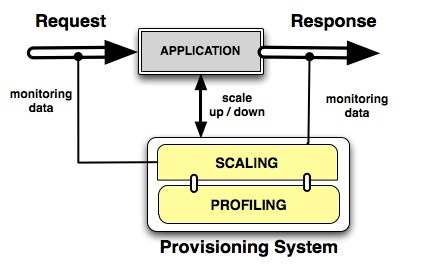
\includegraphics[width=0.4\textwidth, height=4cm]{./images/monitoringSchema.jpg}
\end{center}
\caption{Profiling Resource Provisioning}
\end{figure}
